\documentclass[preprint,12pt,eqsecnum,nofootinbib,amsmath,amssymb]{revtex4}

% Date file was last changed:
\newcommand{\datechange}{3/4/2020}
\newcommand{\datestart}{3/4/2020}

% version
\newcommand\draftverson{v1.5}
\newcommand{\fname}{C\_symmetry\_notes1.5.tex}
\newcommand{\laurnumber}{\draftverson  ~\today ~\currenttime}
\newcommand{\mydate}{\datechange}

% Person who last changed file:>
\newcommand{\whochange}{Robert Singleton}
%
% Project Name, path, informal author names, title
\newcommand{\projname}{Clog Doc}
\newcommand{\dirname}{Clog/doc/dedx}
\newcommand{\myauthors}{Robert Singleton}
\newcommand{\myrunningtitle}{\fname}
\newcommand{\mytitle}{C-Symmetry Notes}



% printing margins
%
\textwidth=6.5in
\textheight=9.5in

% packages
%
\usepackage{graphicx}  % Include figure files
\usepackage{dcolumn}  % Align table columns on decimal point
\usepackage{bm}             % Bold math: $\bm{\alpha}$
\usepackage{latexsym}  % Several additional symbols
\usepackage{fancyhdr}  % Fancy header package
\usepackage{wrapfig}
\usepackage{comment}
\usepackage{dsfont}
\usepackage{mathtools}
\usepackage{datetime}
%\usepackage{showkeys}% Displays equation and fig names
%\usepackage{hyperref}% Hyperlinked references

% local commands
\newcommand{\overoverline}[1]{ {\overline{\overline{#1}}} }
\newcommand{\EMPTYSET}{\varnothing}
\newcommand{\PROOF}{{\tiny PROOF}}
\newcommand{\ALTPROOF}{{\tiny ALTERNATE PROOF}}
\newcommand{\PAR}{$\blacktriangleright$}
\newcommand{\ENDPF}{$\blacksquare$}
\newcommand{\ENDPROOF}{$\blacksquare$}
%\newcommand{\ENDPF}{\square}
%\newcommand{\ENDPROOF}{$\square$}
\newcommand{\AND}{\wedge}
\newcommand{\OR}{\vee}
\newcommand{\NOT}{\neg}
\newcommand{\EQ}{\equiv}
\newcommand{\IFF}{\leftrightarrow}
\newcommand{\IMP}{\rightarrow}
\newcommand{\T}{{\rm T}}
\newcommand{\F}{{\rm F}}
\newcommand{\LOGEQ}{\sim}
\newcommand{\smDash}{{\rule[1mm]{0.1cm}{0.1mm}}}
\newcommand{\dbar}{{d\hskip-0.12cm \rule[2.2mm]{0.15cm}{0.1mm}}}
\newcommand{\smA}{{\scriptscriptstyle \rm A}}
\newcommand{\smB}{{\rm\scriptscriptstyle B}}
\newcommand{\smN}{{\rm\scriptscriptstyle N}}
\newcommand{\smX}{{\rm\scriptscriptstyle X}}
\newcommand{\bvec}[1]{\mathbf{#1}}
\newcommand{\smP}{{\rm\scriptscriptstyle P}}
\newcommand{\smL}{{\rm\scriptscriptstyle L}}
\newcommand{\smT}{{\rm\scriptscriptstyle T}}
\newcommand{\smC}{{\rm\scriptscriptstyle C}}
\newcommand{\smI}{{\rm\scriptscriptstyle I}}
\newcommand{\smR}{{\rm\scriptscriptstyle R}}
\newcommand{\smS}{{\rm\scriptscriptstyle S}}
\newcommand{\smQ}{{\rm\scriptscriptstyle Q}}
\newcommand{\smD}{{\rm\scriptscriptstyle D}}
\newcommand{\smO}{{\rm\scriptscriptstyle 0}}
\newcommand{\smW}{{\rm\scriptscriptstyle W}}
\newcommand{\smCT}{{\rm\scriptscriptstyle CT}}
\newcommand{\smQM}{{\rm\scriptscriptstyle QM}}
\newcommand{\smRe}{{\rm\scriptscriptstyle Re}}
\newcommand{\smIm}{{\rm\scriptscriptstyle Im}}
\newcommand{\smFe}{{\rm\scriptscriptstyle Fe}}
\newcommand{\smCL}{{\rm\scriptscriptstyle CL}}
\newcommand{\smBPS}{{\rm\scriptscriptstyle BPS}}
\newcommand{\smAMU}{{\rm\scriptscriptstyle AMU}}
\newcommand{\smE}{{\rm\scriptscriptstyle E}}
\newcommand{\smae}{{\rm\scriptscriptstyle ae}}
\newcommand{\extend}[2]{ {#1}^\smallfrown{\! #2} }
\newcommand{\smTC}{{\rm\scriptstyle TC}}
\newcommand{\calT}{ {\cal T}}
\newcommand{\calA}{{\cal A}}
\newcommand{\mathfrakA}{\mathfrak{A}}
\newcommand{\mathfrakB}{\mathfrak{B}}
\newcommand{\mathfrakS}{\mathfrak{S}}
\newcommand{\smGr}{{\rm\scriptscriptstyle gr}}
\newcommand{\smLT}{{\rm\scriptscriptstyle <}}
\newcommand{\smGT}{{\rm\scriptscriptstyle >}}
\newcommand{\smY}{{\rm\scriptscriptstyle Y}}

% % baselineskip modes
\newcommand{\bodyskip}{\baselineskip 18pt plus 1pt minus 1pt}
\newcommand{\bibskip}{\baselineskip16pt plus 1pt minus 1pt}
\newcommand{\tableofcontentsskip}{\baselineskip 14pt plus 1pt minus 1pt}
\newcommand{\footnoteskip}{\baselineskip 12pt plus 1pt minus 1pt}
\newcommand{\abstractskip}{\baselineskip 13pt plus 1pt minus 1pt}
\newcommand{\titleskip}{\baselineskip 18pt plus 1pt minus 1pt}
\newcommand{\affiliationskip}{\baselineskip 15pt plus 1pt minus 1pt}
\newcommand{\captionskip}{\footnotesize \baselineskip 12pt plus 1pt minus 1pt}
\newcommand{\enumerateskip}{\baselineskip 14pt plus 1pt minus 1pt}
\newcommand{\theoremskip}{\baselineskip 13pt plus 1pt minus 1pt}

% theorem
%
\newtheorem{theorem}{Theorem}
\newtheorem{corollary}[theorem]{Corollary}
\newtheorem{definition}[theorem]{Definition}
\newtheorem{lemma}[theorem]{Lemma}
\newtheorem{proposition}[theorem]{Proposition}
\newtheorem{example}[theorem]{Example}
%\newtheorem{theorem}{Theorem}
%\newtheorem{corollary}{Corollary}
%\newtheorem{definition}{Definition}

\pagestyle{fancy}
\lhead{\laurnumber}
%\lhead{}
\chead{}
\rhead{}
\lfoot{}
\cfoot{\thepage}
\rfoot{}

%%
%% begin: draw box
%%
%%%%%%%%%%%%%%%%%%%%%%%%%%%%%%
%%
%%  This macro draws a box around around text, taken 
%%  from ``TeX by Example'', by Arvind Borde p76.
%%
%%   To use: 
%%
%%   \vskip0.3cm
%%   \frame{.1}{2}{16.2cm}{\noindent
%%   \begin{eqnarray}
%%     a = b
%%   \end{eqnarray}
%%   }
%%   \vskip0.2cm
%%
%%%%%%%%%%%%%%%%%%%%%%%%%%%%%%%
%%
\def\frame#1#2#3#4{\vbox{\hrule height #1pt    % TOP RULE
  \hbox{\vrule width #1pt\kern #2pt                     % RULE/SPACE ON LEFT
  \vbox{\kern #2pt                                               % TOP SPACE
  \vbox{\hsize #3\noindent #4}                            % BOXED MATERIAL
  \kern #2pt}                                                        % BOTTOM SPACE
  \kern #2pt\vrule width #1pt}                              % RULE/SPACE ON RIGHT
  \hrule height0pt depth #1pt}                            % BOTTOM RULE
}
%%
\def\myframe#1{\vbox{\hrule height 0.1pt    % TOP RULE
  \hbox{\vrule width 0.1pt\kern 2pt                     % RULE/SPACE ON LEFT
  \vbox{\kern 2pt                                               % TOP SPACE
  \vbox{\hsize 16.5cm\noindent #1}                            % BOXED MATERIAL
  \kern 2pt}                                                        % BOTTOM SPACE
  \kern 2pt\vrule width 0.1pt}                              % RULE/SPACE ON RIGHT
  \hrule height0pt depth 0.1pt}                            % BOTTOM RULE
}
%%
%% draws two boxes around text (use sparingly)
%%
\def\fitframe #1#2#3{\vbox{\hrule height#1pt  % TOP RULE
  \hbox{\vrule width#1pt\kern #2pt             % RULE/SPACE ON LEFT
  \vbox{\kern #2pt\hbox{#3}\kern #2pt}         % TOP,MATERIAL,BOT
  \kern #2pt\vrule width#1pt}                  % RULE/SPACE ON RIGHT
  \hrule height0pt depth#1pt}                  % BOTTOM RULE
}
%%
%% draws a box with shadow around text
%%
\def\shframe #1#2#3#4{\vbox{\hrule height 0pt % NO TOP SHADOW
 \hbox{\vrule width #1pt\kern 0pt             % LEFT SHADOW
 \vbox{\kern-#1pt\frame{.3}{#2}{#3}{#4}       % START SHADOW
 \kern-.3pt}                                  % MOVE UP RULE
 \kern-#2pt\vrule width 0pt}                  % STOP SHADOW
 \hrule height #1pt}                          % BOTTOM SHADOW
}
%%
%%
%% end: draw box
%%
%%  To install as a package on a local host.
%%   a. Append the header ``\usepackage{myboxes}'' to the above macro. Name 
%%   the macreo file myboxes.sty.  Move myboxes.sty into $HOME/texmf/tex/mypackages/. 
%%   You might need to type texhash.
%%   b. T use the package write \usepackage{myboxes} in the preamble.

%
\begin{document}

%% notes info page
%\hfill{\laurnumber}
%\vskip0.3cm
\centerline{{ \Large\bf \projname: \fname}}
\vskip0.25cm 
\centerline{\bf \mytitle}
\vskip0.25cm
\centerline{\myauthors}
\vskip0.75cm 
\baselineskip 14pt plus 1pt minus 1pt
\begin{flushright}
Research Notes   \\[3pt]
{\it Project}:          \\
\projname                      \\
  {\it Path of TeX Source}:          \\
\dirname/\fname                      \\[3pt]
{\it Last Modified By}:            \\
\whochange                         \\
\datechange                        \\[3pt]
{\it Date Started:}                \\
\datestart                         \\[3pt]
{\it Date:}                \\
\draftverson~ \today ~\currenttime \\
\end{flushright}

\baselineskip 20pt plus 1pt minus 1pt

%% mini abstract
%\abstractskip
%\noindent
%These are notes on Logic from Ref.~\cite{ref_chang}.  
%\bodyskip

%% title page
\vskip2.0cm
%\pagebreak
\preprint{\laurnumber}

% publication title page
\title{\titleskip
  \mytitle
}

\author{Robert L Singleton Jr}

\affiliation{\affiliationskip
   School of Mathematics\\
   University of Leeds\\
   LS2 9JT
}

\date{\datechange}

\begin{abstract}
\abstractskip
\vskip0.3cm 
\noindent
  Physics documentation for the BPS temperature equilibration in the code Clog.
\end{abstract}

%%
\maketitle
%%

% to change page settings
%\thispagestyle{empty}
%\pagestyle{empty}
%\setcounter{page}{0}

\pagebreak
\tableofcontentsskip
\tableofcontents
%\thispagestyle{empty}

%\pagebreak
\newpage
\bodyskip
%\setcounter{page}{1}

\pagebreak
\clearpage

\newpage
\section{The Symmetry Condition
}

\subsection{Statement of the Problem}

We consider a plasma with component species labeled by $a$ and $b$,
each in local thermodynamic equilibrium among themselves (but not each
other) with respective temperatures $T_a$ and $T_b$. The rate of
energy exchange per unit volume {\em from} the $a$-subsystem {\em to}
the $b$-subsystem takes the form
%%
\begin{eqnarray}
  \frac{d{\cal E}_{ab}}{dt} 
  = 
  -\,{\cal C}_{ab}\,\Big(T_a - T_b \Big) \ ,
\label{dEdtabIntro}
\end{eqnarray}
%% 
which serves to define the rate coefficients ${\cal C}_{ab}$. Energy
conservation, which can be written in the form $d{\cal E}_{ab}/dt =
-d{\cal E}_{ba}/dt$, implies the symmetry of the rate coefficient
itself
%%
\begin{eqnarray}
  {\cal C}_{ab}={\cal C}_{ba} \ .
\end{eqnarray}
%% 
On the other hand, from Eq.~(12.3) of BPS, the rate coefficients can
be expressed as
%%
\begin{eqnarray}
  {\cal C}_{ab} 
  &=& 
  \int \frac{d^3 p_a}{(2\pi\hbar)^3}\, f_a({\bf p}_a)\,
  \beta_a v_a\,{\cal A}_{ab}({\bf p}_a) 
\label{CabIntro}
\\[5pt]
  &=&
  \frac{2 n_a\, c\, \beta_a^{5/2}}{\sqrt{m_ac^2\,}}\,
  \sqrt{\frac{2}{\pi}} \! \int_0^\infty \! dE\,E\, e^{-\beta_a E} \,
  {\cal A}_{ab}(E) \ .
\label{CabIntroAlg}
\end{eqnarray}
%% 
We will derive this latter form in another section, but for now it
suffices to note that we have only used the Maxwell-Boltzmann
distribution (\ref{fadefEa}), along with spherical symmetry in
momentum to express $f_a$ and ${\cal A}_{ab}$ in terms of energy
$E=p_a^2/2m_a$. The symmetry of (\ref{CabIntro}) or
(\ref{CabIntroAlg}) under the interchange $a \leftrightarrow b$ is
hardly evident, and the purpose of these notes is to explain this
seeming puzzle.


We can express the problem in another form. Suppose the ions are in
equilibrium among themselves at some temperature $T_\smI$, and suppose
the electron temperature is $T_e$. Letting the first index of
(\ref{dEdtabIntro}) correspond to the electron, and upon summing over
the ions in the second index, the rate equation becomes
%%
\begin{eqnarray}
  \frac{d{\cal E}_{e\smI}}{dt} 
  = 
  -\,{\cal C}_{e\smI}\,\Big(T_e - T_\smI \Big) \ ,
\label{dEdteIIntro}
\end{eqnarray}
%% 
\noindent
where ${\cal C}_{e\smI}={\sum}_i { \cal C}_{ei}$ and $d{\cal
  E}_{e\smI}/dt={\sum}_i d{ \cal E}_{ei}/dt$. As before, energy
conservation (treating the ions as a single subsystem) implies that
${\cal C}_{e\smI}$ is symmetric under $e \leftrightarrow {\rm I}$. The
advantage of the form (\ref{dEdteIIntro}), however, is that the rate
coefficient greatly simplifies in the extreme quantum limit ($\eta \to
0$). Since the electron is so light, the calculational trick is to
employ a sum-rule that emerges from the $m_e/m_\smI \to 0$ limit,
from which a quite simple result emerges, 
%%
\begin{eqnarray}
\nonumber
  && m_e/m_\smI \to 0 \,,\, \eta \to 0: \\[5pt]
  && 
  {\cal C}_{e\smI} 
  = 
  \underbrace{~
  \frac{\kappa_e^2}{2\pi}\,
  \left(\frac{\beta_e m_e}{2\pi} \right)^{1/2} \omega_\smI^2 
  ~}_\text{prefactor}
  \cdot
  \underbrace{~
  \frac{1}{2} \left[ \ln\left\{ \frac{8 T_e^2}{\hbar^2 \omega_e^2}
  \right\} -\gamma -1 \right] 
  ~}_{\text{Coulomb Log:} \ln\Lambda_\smBPS^{\smQM}} 
  \ ,
\end{eqnarray}
%% 
\noindent
where $\omega_\smI^2 = {\sum}_i \omega_i^2$.  We will use rationalized
cgs units (the Coulomb potential is $V=e^2/4\pi r$) for which the
Debye wavenumber and the plasma frequency take the form
%%
\begin{eqnarray}
  \kappa_a^2 &=& \frac{e_a n_a}{T_a}
\\[5pt]
  \omega_a^2 &=& \frac{e_a n_a}{m_a} \ ;
\end{eqnarray}
%% 
the electron plasma coupling is given by
%%
\begin{eqnarray}
  g_e = \frac{e^2 \kappa_e}{4\pi\, T_e} \ .
\end{eqnarray}
%% 

\subsection{Realizing a Two-Temperature Plasma in Nature}

In these notes we consider a two-temperature plasma for which the
electrons and ions have temperatures $T_e$ and $T_\smI$,
respectively. The most direct way to realize this in nature is a
two-component plasma, that is to say, a plasma with with electrons of
mass $m_e$ and a {\em single} species of ion with mass
$m_\smI$. Because the electron is thousands of times lighter than an
ion, collisions between the electrons will rapidly bring the electron
sub-system into equilibrium with itself at some temperature $T_e$;
soon thereafter the ions will equilibrate to different common
temperature $T_\smI$ (at a rate $\sqrt{m_e/m_\smI}$ slower than
electron equilibration). Finally, the electron-ion system begins to
exchange Coulomb energy and starts to equilibrate according to
(\ref{dEdtabIntro})

In fact, the form (\ref{dEdtabIntro}) expresses the Coulomb energy exchange
between any number of species in a multi-component plasma [$a,b \in
\{1, 2, \cdots, N \}$\,], provided each species maintains local
thermodynamic equilibrium with itself at a well defined
temperature. This hypothetical scenario is physically realized in a
plasma with multiple, well-separated, mass scales. For example,
consider a Deuterium-Tritium (DT) plasma: the electrons will
equilibrate to a temperature $T_e$ and the DT to a common temperature
$T_\smI$. If this plasma also contained a heavy large-$Z$ species,
such as iron, then this component will equilibrate to some temperature
$T_\smFe$ soon after the D-T equilibration, although we will not
consider the three-temperature case. 

\subsection{The Rate Coefficient}

Let's now use the fact that $f_a$ and ${\cal A}_{ab}$ are radially
symmetric in their momentum argument to change variables in
(\ref{CabIntro}) to energy $E_a = p_a^2/2 m_a$:
%%
\begin{eqnarray}
  {\cal C}_{ab} 
  &=& 
  \frac{4\pi}{(2\pi\hbar)^3}\!
  \int_0^\infty \!\! p_a^2 dp_a\, f_a(E_a)\,
  \frac{\beta_a p_a}{m_a}\,{\cal A}_{ab}(E_a) 
  =
  \frac{4\pi\,\beta_a}{(2\pi\hbar)^3}\!
  \int_0^\infty \!\!
  (2 m_a E_a) d (p_a^2/2 m_a) f_a(E_a)\,{\cal A}_{ab}(E_a) 
\nonumber
\\[5pt]
  &=&
  \frac{8\pi\,\beta_a m_a}{(2\pi\hbar)^3}\int_0^\infty \! 
  d E_a\, E_a \, f_a(E_a)  {\cal A}_{ab}(E_a) \ .
\label{Cabintradial}
\end{eqnarray}
%%
The distribution function is expressed by Eq.~(7.4) of BPS, and
in terms of energy $E_a$ we can write
%%
\begin{eqnarray}
  f_a(E_a) 
  = 
  n_a \left(\frac{2\pi \hbar^2 \beta_a}{m_a}
  \right)^{3/2} e^{-\beta_a E_a}   \ .
\label{fadefEa}
\end{eqnarray}
%% 
This gives the rate coefficient,
%%
\begin{eqnarray}
  {\cal C}_{ab} 
  &=& 
  \frac{8\pi\,\beta_a m_a}{(2\pi\hbar)^3}\int_0^\infty \! 
  d E_a\, E_a \cdot   n_a \left(\frac{2\pi \hbar^2 \beta_a}{m_a}
  \right)^{3/2} e^{-\beta_a E_a}   \cdot {\cal A}_{ab}(E_a) \ ;
\end{eqnarray}
%%
changing the dummy integration variable from $E_a$ to $E$, and
combining terms in the prefactor gives
%%
\begin{eqnarray}
  {\cal C}_{ab} 
  &=& 
  \frac{2 n_a\, \beta_a^{5/2}}{\sqrt{m_a}} \cdot
  \sqrt{\frac{2}{\pi}}
  \int_0^\infty \! 
  d E\, E\,    e^{-\beta_a E}\, {\cal A}_{ab}(E) \ .
\end{eqnarray}
%%
It is useful to change the integration variable to the dimensionless
quantity $x = \beta_a E$, thereby giving
%%
\begin{eqnarray}
  \int_0^\infty \! 
  d E\, E\,    e^{-\beta_a E}\, {\cal A}_{ab}(E) 
  =
  \frac{1}{\beta_a^2}\int_0^\infty \! 
  d x\, x\,    e^{-x}\, {\cal A}_{ab}(x/\beta_a) \ .
\end{eqnarray}
%%
The coefficient can now be written
%%
\vskip0.2cm 
\frame{.1}{2}{16.4cm}{\noindent
\begin{eqnarray}
  {\cal C}_{ab} 
  &=& 
  \frac{2\,n_a\, c}{\sqrt{T_a\,m_a c^2\,}} 
  \cdot
  \sqrt{\frac{2}{\pi}}
  \int_0^\infty \! 
  d x\, x\,    e^{-x}\, {\cal A}_{ab}(T_a\,x) \ .
\end{eqnarray}
}
%%
\noindent
Units: $[n c /\text{Energy}] \cdot [{\cal A}]=
{\rm cm}^{-3} \cdot ({\rm cm/s}) \cdot \text{Energy}^{-1} 
\cdot (\text{Energy}/{\rm cm})={\rm cm^{-3}}\cdot s^{-1}$. 

\vskip0.3cm
\noindent
For a single-ion plasma such as a hydrogen plasma, this becomes
%%
\begin{eqnarray}
  {\cal C}_{e\smI}^\text{dist} 
  &=& 
  \underbrace{~
  \frac{2\, n_e\,c}{\sqrt{T_e\,m_e c^2\,}}
  ~}_{\text{prefactor}~N_e} 
  \cdot
  \underbrace{~
  \sqrt{\frac{2}{\pi}}
  \int_0^\infty \! 
  d x\, x\,    e^{-x}\, {\cal A}_{e\smI}(T_e\,x)
  ~}_{\text{integral}~ {\bar C_{e\smI}}   } \ ,
\end{eqnarray}
%%
where the superscript ``dist'' now indicates that the rate coefficient
has been calculated using the distribution function relation. The
rescaled integrand $\bar C_{e\smI}(x) = \sqrt{\frac{2}{\pi}}\, x
\,e^{-x} {\cal A}_{e\smI}(T_e\,x)$ is plotted below for the
temperatures $T_e=T_\smI=10\,{\rm keV}$ and $T_e=T_\smI=100\,{\rm
keV}$.


\pagebreak
%%

~

%\vskip-2.0cm 
\begin{figure}[h!]
%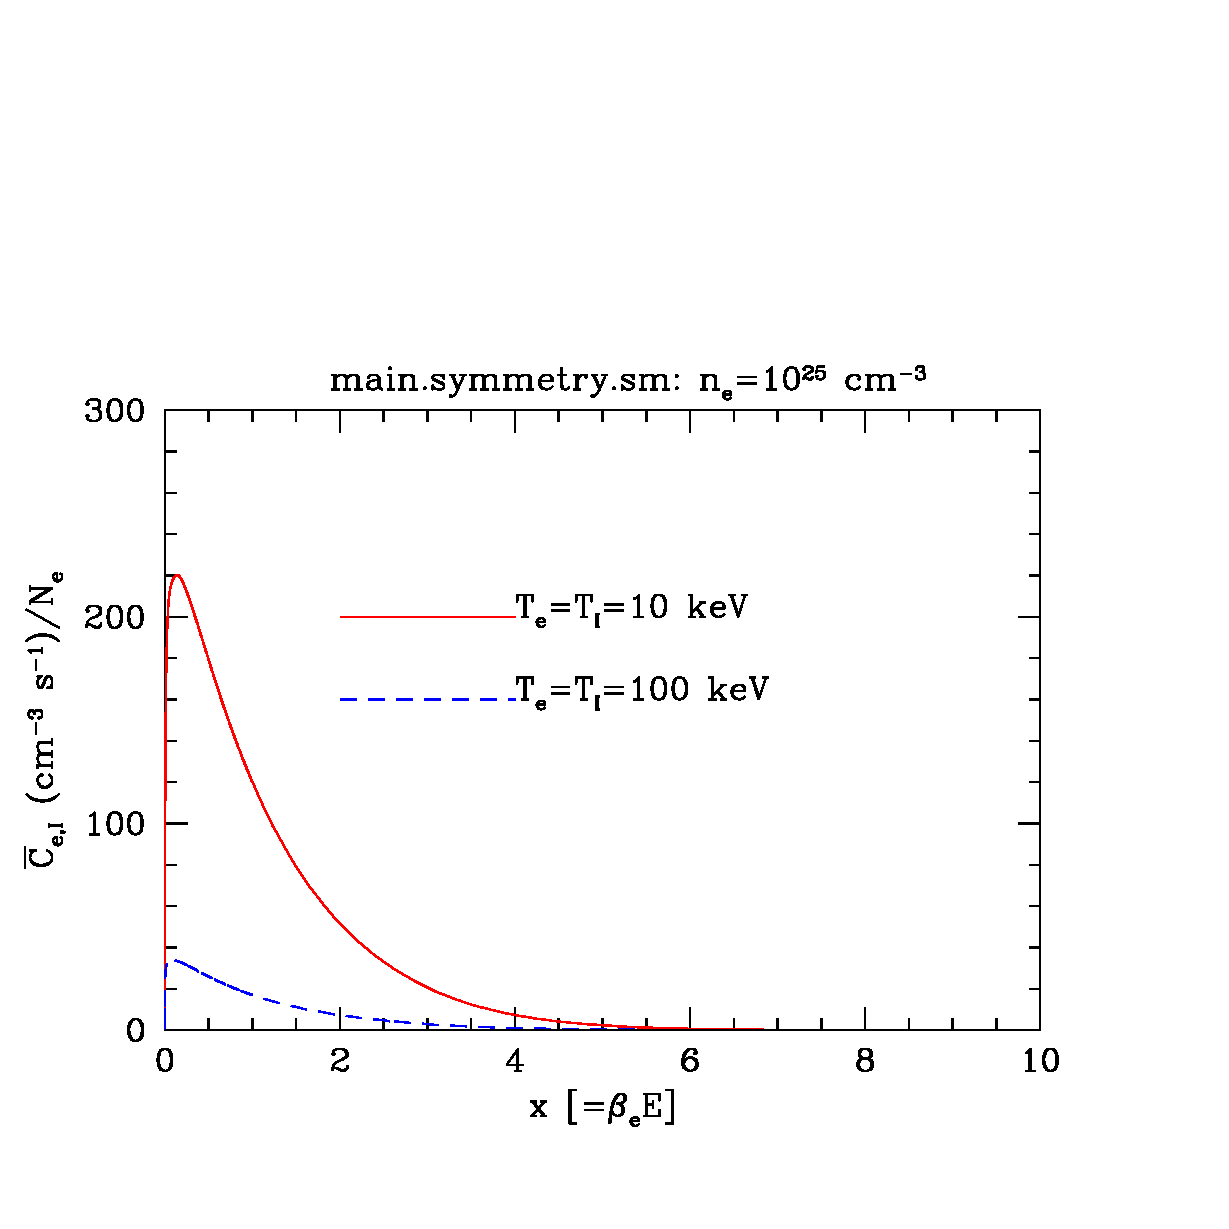
\includegraphics[scale=0.45]{main.symmetry.eps} 
\vskip-0.3cm 
\caption{\footnoteskip  
%% 
  The integrand $\bar C_{e\smI}(x)=\sqrt{2/\pi}\, x\, e^{-x} {\cal
  A}_{e\smI}(T_e x) $ for a hydrogen plasma with $n_e= 10^{25}\,{\rm
  cm}^{-3}$ for electron-ion temperatures of $T_e=T_\smI=10\,{\rm
  keV}$ (red solid) and $T_e=T_\smI=100\,{\rm keV}$ (blue dashed).
  See the table for numerical values. [main.symmetry.f90,
  main.symmetry.sm, main.symmetry.010kev.dat,
  main.symmetry.100kev.dat, main.symmetry.eps]
%%
}
\label{fig:main.symmetry.eps}
\end{figure}
%%
\noindent
This integrand turns out to be difficult to numerically integrate, and
the problem with the integral will turn out to lie with the small mass
ratio. The next figure plots the rescaled integrand $\bar C_{e\smI}(x)
= \sqrt{\frac{2}{\pi}}\, x \,e^{-x} {\cal A}_{e\smI}(T_e\,x)$ in the
region of small-$x$:

~

%%
%\vskip-3.0cm 
\begin{figure}[h!]
%\includegraphics[scale=0.45]{main.symmetry.smallE.eps} 
\vskip-0.3cm 
\caption{\footnoteskip  
%% 
  Same as Fig.~\ref{fig:main.symmetry.eps}, except $x$-axis runs over
  $[0,0.01]$. 
%%
}
\label{fig:main.symmetry.smallE.eps}
\end{figure}
%%

~

\noindent
The dip in the 10\,keV case suggest that we will have to break
the interval into small regions, and we may even be required to
use the small-E asymptotic form for ${\cal A}_{ab}$. 



%\pagebreak
\noindent
In the following table we illustrate the integral $\bar C_{e\smI} =
\int_0^{x_\text{max}} \!  dx\, \bar C_{e\smI}(x)$. The integration
problem crops up immediately, as errors of order 15--20\% are far too
large.

%
% A Table with figure caption at the top
%
%%
~
\begin{table}[hb!]
\caption{\footnoteskip 
%%
  Rate coefficients with $x_\text{max}=30$ with $N=1000$
%%
}
\begin{tabular}{|l||c|c|} \hline
   ~${\cal C}_{e\smI} ~~{\rm [cm^{-3} \,s^{-1}] }$~ & ~$T_e=T_\smI=10\,{\rm keV}$~     & ~$T_e=T_\smI=100\,{\rm keV}$~\\ \hline
   ~${\cal C}_{e\smI}^\text{\,sum-rule}$~             & ~$2.228 \times 10^{36}$~         & ~$1.050 \times 10^{35}$~     \\
   ~${\cal C}_{e\smI}^\text{\,exact}$~                & ~$2.220 \times 10^{36}$~         & ~$1.048 \times 10^{35}$~     \\
   ~${\cal C}_{e\smI}^\text{\,dist}$~                 & ~$2.612 \times 10^{36}$~         & ~$1.194 \times 10^{35}$~     \\\hline\hline
   ~$\bar{\cal C}_{e\smI} $~                        &      & \\\hline
   ~$\bar{\cal C}_{e\smI}^\text{\,sum-rule}$~         & ~265.7~         & ~39.6~     \\
   ~$\bar{\cal C}_{e\smI}^\text{\,exact}$~            & ~264.7~         & ~39.5~     \\
   ~$\bar{\cal C}_{e\smI}^\text{\,dist}$~             & ~311.5~         & ~45.0~     \\\hline
   ~\% error~                                         & ~18\%~          & ~14\%~     \\\hline
\end{tabular} 
\label{table:fractALP1}
\end{table}
%%

\noindent
Note that the sum-rule and the exact results are almost the same, and
therefore the sum rule is a good approximation in these plasma
regimes. The distribution function result is about 20\% too high;
however, the next table shows that we can do much better and the large
error is a numerical artifact.


~
\vskip-0.3cm 
\begin{table}[hb!]
\caption{\footnoteskip 
%%
  Rate coefficients using four smaller integration intervals: $[0,
  0.2]$, $[0.2,1]$, $[1,3]$, and $[3,30]$, with $N=1000$ in each interval.
%%
}
\begin{tabular}{|l||c|c|} \hline
   ~${\cal C}_{e\smI} ~~{\rm [cm^{-3} \,s^{-1}] }$~ & ~$T_e=T_\smI=10\,{\rm keV}$~     & ~$T_e=T_\smI=100\,{\rm keV}$~\\ \hline
   ~${\cal C}_{e\smI}^\text{\,sum-rule}$~             & ~$2.228 \times 10^{36}$~       & ~$1.050 \times 10^{35}$~     \\
   ~${\cal C}_{e\smI}^\text{\,exact}$~                & ~$2.220 \times 10^{36}$~       & ~$1.049 \times 10^{35}$~     \\
   ~${\cal C}_{e\smI}^\text{\,dist}$~                 & ~$2.248 \times 10^{36}$~       & ~$1.013 \times 10^{35}$~     \\\hline\hline
   ~$\bar{\cal C}_{e\smI} $~                        &      & \\\hline
   ~$\bar{\cal C}_{e\smI}^\text{\,sum-rule}$~         & ~265.7~         & ~39.6~     \\
   ~$\bar{\cal C}_{e\smI}^\text{\,exact}$~            & ~264.7~         & ~39.5~     \\
   ~$\bar{\cal C}_{e\smI}^\text{\,dist}$~             & ~268.0~         & ~38.2~     \\\hline
   ~\% error~                                         & ~1.3\%~         & ~3.4\%~     \\\hline
\end{tabular} 
\label{table:fractALP2}
\end{table}
%%

\noindent
Let's check the extent to which the accuracy problem arises from the
extremely small mass ratio $m_e/m_\smI$ by setting the electron mass
to half the proton mass, $m_e = \frac{1}{2}\, m_p$. In this case, the
sum-run results should not be accurate, but the other two methods
(exact and distribution function) should agree.

\vskip-2.0cm 
\begin{figure}[h!]
%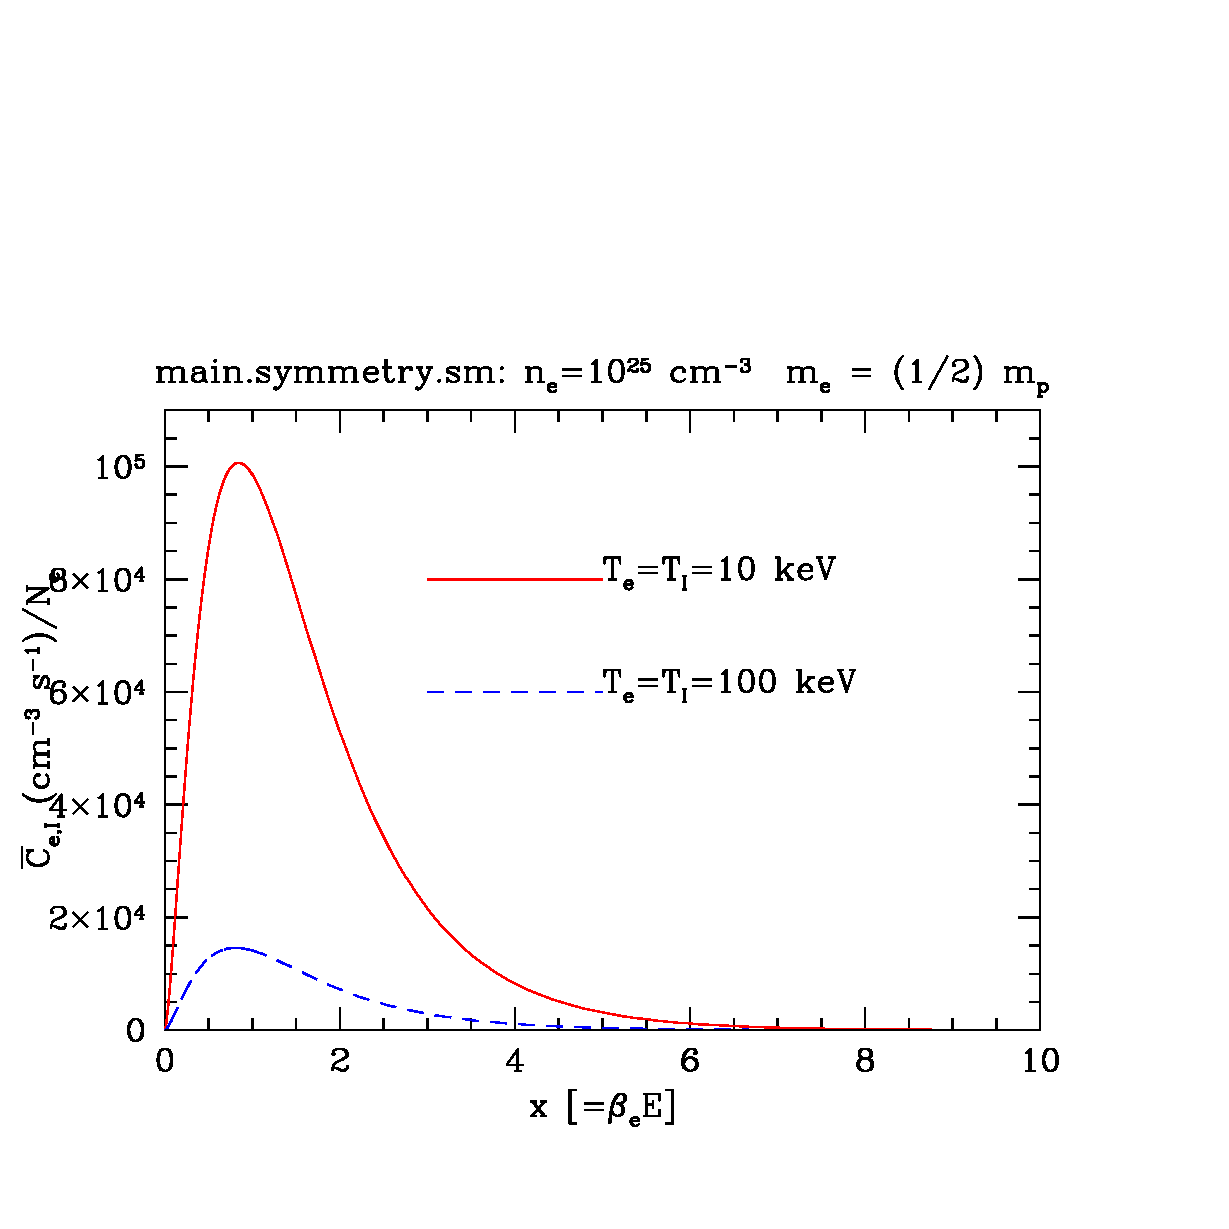
\includegraphics[scale=0.45]{main.symmetry.heavyMe.eps} 
\vskip-0.3cm 
\caption{\footnoteskip  
%% 
  The integrand $\bar C_{e\smI}(x)=\sqrt{2/\pi}\, x\, e^{-x} {\cal
  A}_{e\smI}(T_e x)$ with a heavy electron. [main.symmetry.f90, \\
  main.symmetry.heavyMe.sm, main.symmetry.heavyMe.010kev.dat, 
  main.symmetry.heavyMe.100 kev.dat, main.symmetry.heavyMe.eps]
%%
}
\label{fig:main.symmetry.heavyMe.eps}
\end{figure}
%%


~
\vskip-0.3cm 
\begin{table}[hb!]
\caption{\footnoteskip 
%%
    Rate coefficients setting $m_e=\frac{1}{2}\, m_p$ with an interval
    $[1,30]$ and $N=1000$. 
%%
}
\begin{tabular}{|l||c|c|} \hline
   ~${\cal C}_{e\smI} ~~{\rm [cm^{-3} \,s^{-1}] }$~ & ~$T_e=T_\smI=10\,{\rm keV}$~     & ~$T_e=T_\smI=100\,{\rm keV}$~\\ \hline
   ~${\cal C}_{e\smI}^\text{\,sum-rule}$~             & ~$11.65 \times 10^{37}$~       & ~$4.733 \times 10^{36}$~     \\
   ~${\cal C}_{e\smI}^\text{\,exact}$~                & ~$5.676 \times 10^{37}$~       & ~$2.523 \times 10^{36}$~     \\
   ~${\cal C}_{e\smI}^\text{\,dist}$~                 & ~$5.729 \times 10^{37}$~       & ~$2.545 \times 10^{36}$~     \\\hline\hline
   ~$\bar{\cal C}_{e\smI} $~                        &      & \\\hline
   ~$\bar{\cal C}_{e\smI}^\text{\,sum-rule}$~         & ~421094~         & ~54069~     \\
   ~$\bar{\cal C}_{e\smI}^\text{\,exact}$~            & ~205068~         & ~28826~     \\
   ~$\bar{\cal C}_{e\smI}^\text{\,dist}$~             & ~206980~         & ~29073~     \\\hline
   ~\% error~                                         & ~0.9\%~         & ~0.86\%~     \\\hline
\end{tabular} 
\label{table:fractAL3}
\end{table}
%%



\pagebreak
\clearpage
\section{Low Energy Classical Result}

In A\_asymptotic1.7.tex we calculated the classical and quantum rate
coefficient analytically using the low energy forms. As we see from
Figs.~\ref{fig:gr031}~and~\ref{fig:gr051}, the classical contribution
dominates the low-energy asymptotic form for the ions. We will
therefore calculate the rate using the classical form
%%
\begin{eqnarray}
  {\cal A}_{\smCL,ab}(v_p)
  &=&
  \frac{e_p^2\,\kappa_b^2}{2\pi}\, 
  \left( \frac{\beta_b m_b}{2\pi}\right)^{1/2} v_p \,
  \bar A_b^\smCL
\\
  \bar A_b^\smCL
  &=&
  -\frac{2}{3}\left[\ln\left\{ \frac{e_p e_b \beta_b \kappa_\smD}{16\pi}\,
  \frac{m_b}{m_{pb}}\right\} + \frac{1}{2} + 2 \gamma
  \right] \ ,
\end{eqnarray}
%%
or specializing to ions (and electron projectiles) we have
%%
\begin{eqnarray}
  {\cal A}_{\smCL,e\smI}(v_e)
  &=&
  \frac{e^2\,\omega_\smI^2}{2\pi}\, \beta_\smI m_\smI
  \left( \frac{\beta_\smI m_\smI}{2\pi}\right)^{1/2} 
  \bar A_\smI^\smCL \, v_e
\\
  \bar A_\smI^\smCL
  &=&
  -\frac{2}{3}\left[\ln\left\{ \frac{Z_\smI e^2 \beta_\smI 
  \kappa_\smD}{16\pi}\,\frac{m_\smI}{m_{e\smI}}\right\} + 
  \frac{1}{2} + 2 \gamma \right] \ .
\end{eqnarray}
%%

~

%%
\vskip-2cm 
\begin{figure}[h!]
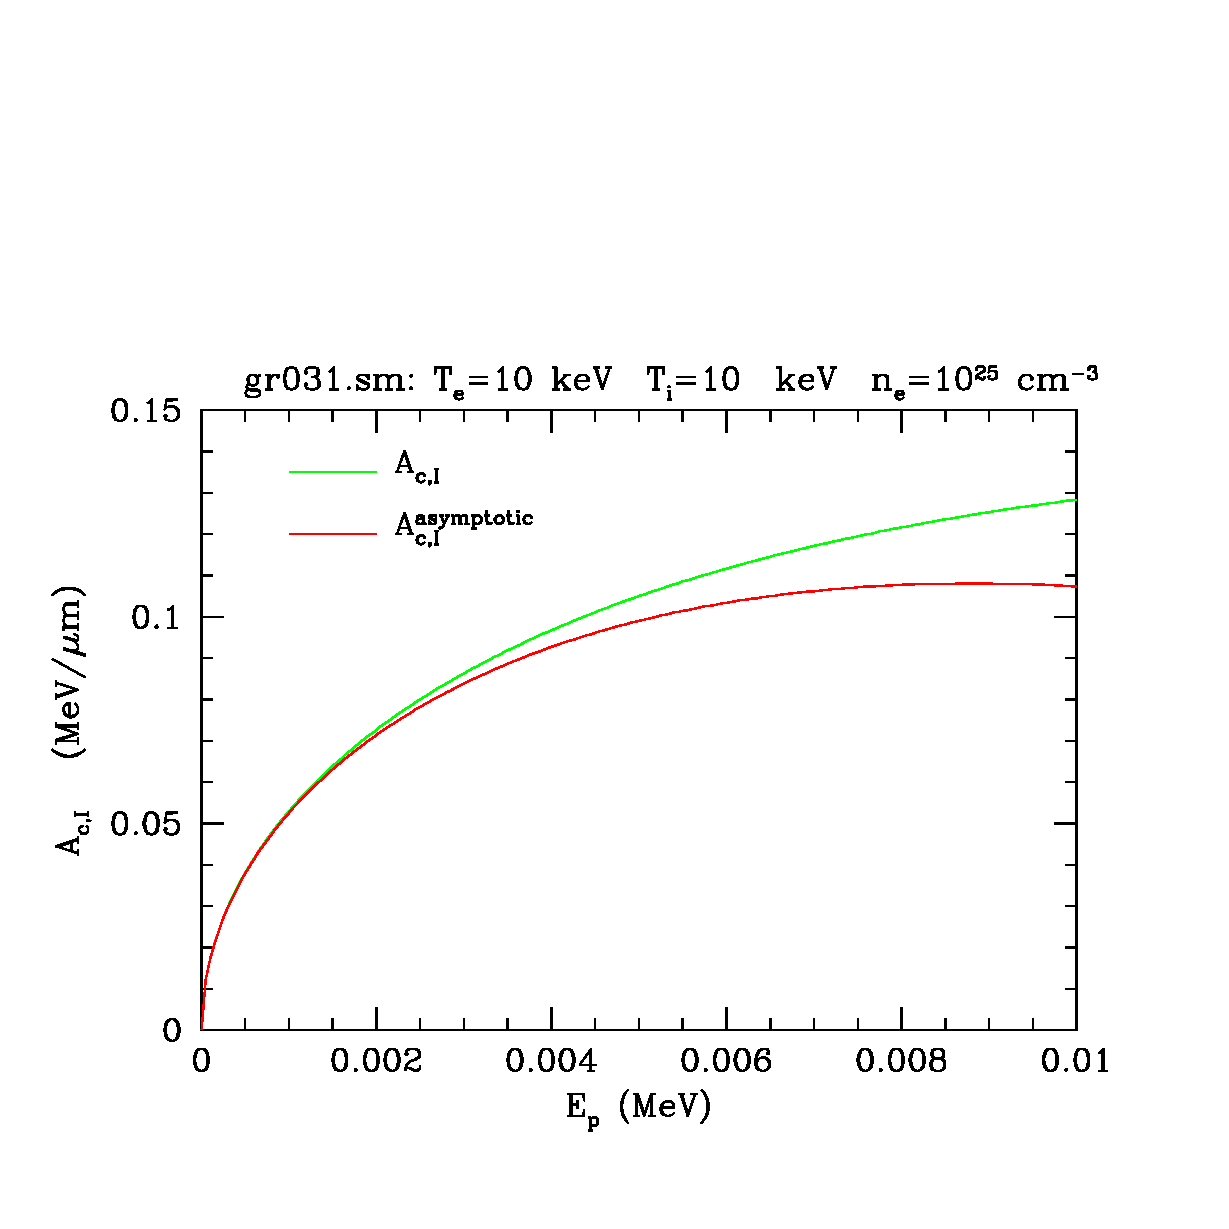
\includegraphics[scale=0.45]{gr031.eps} 
\vskip-0.8cm 
\caption{\footnoteskip  
%%
  Asymptotic classical ion contribution at low energies. [gr001.f90,
  gr031.sm, gr001.dat, gr001.smallE.dat, gr031.eps]
%%
}
\label{fig:gr031}
\end{figure}
%%

~

%%
\vskip-2.0cm 
\begin{figure}[h!]
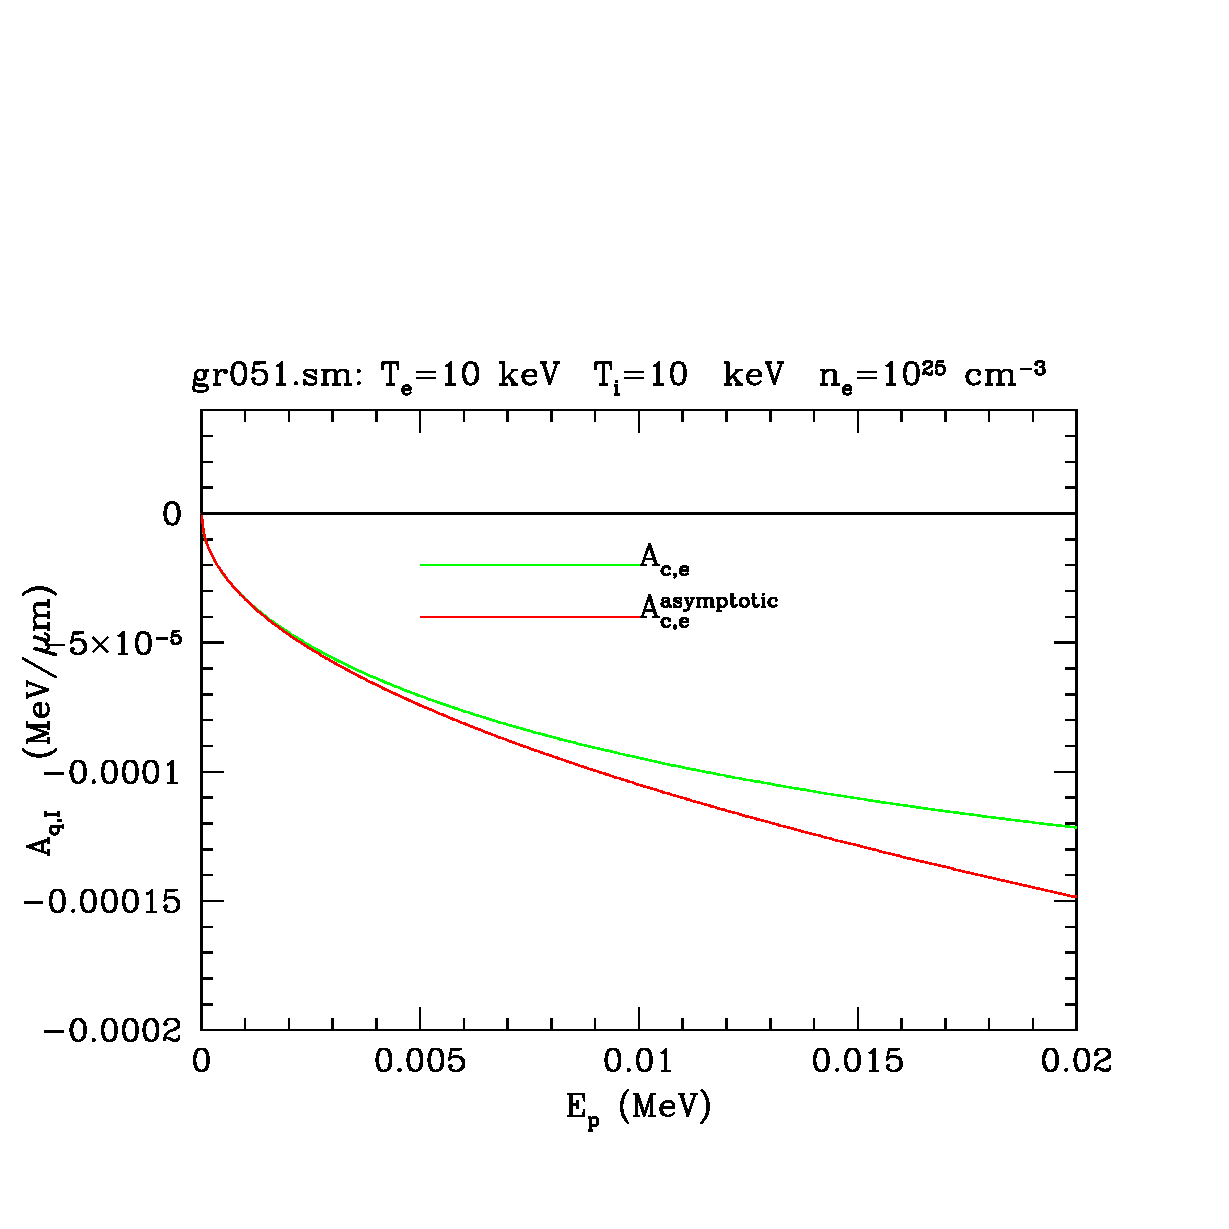
\includegraphics[scale=0.45]{gr051.eps} 
\vskip-0.8cm 
\caption{\footnoteskip  
%%
  Asymptotic quantum ion contribution at low energies. [gr001.f90,
  gr051.sm, gr001.dat, gr001.smallE.dat, gr051.eps]
%%
}
\label{fig:gr051}
\end{figure}
%%

\pagebreak
We need to separate the classical small-E result into its singular and
regular contributions. Equation (9.8) on p.\,300 of BPS gives the
small energy asymptotic form of the singular piece: 
%%
\begin{eqnarray}
  {\cal A}_{ab,\smS}^{\smCL}
  &=&
  \underbrace{~\frac{e_p^2\,\kappa_b^2}{4\pi}~}_{c_1}
  ~
  \underbrace{\left( \frac{\beta_b m_b}{2\pi}\right)^{1/2} v_p}_{
  c_2} 
  \cdot \,
  \bar A_{ab,\smS}^\smCL
\\
  \bar A_{ab,\smS}^\smCL
  &=&
  -\left(\frac{2}{3} - \frac{1}{5}\,\beta_b m_b\,v_p^2 \right)
  \left[\ln\left\{ \frac{e_p \,e_b \beta_b \, K}{16\pi}\,
  \frac{m_b}{m_{pb}}\right\} + 2 \gamma
  \right] 
  + 
  \frac{2}{15}\,\beta_b m_b \, v_p^2  
  +
  {\cal O}(v_p^5)\ ;
\end{eqnarray}
%%
while Eq.~(7.34) on p\,(287) of BPS gives the regular
piece:
%%
\begin{eqnarray}
  {\cal A}_{ab,\smR}^{\smLT} 
  &=&
  \underbrace{~\frac{e_p^2\,\kappa_b^2}{4\pi}~}_{c_1}
  ~
  \underbrace{\left( \frac{\beta_b m_b}{2\pi}\right)^{1/2} v_p}_{
  c_2} 
  \cdot \,
  \bar A_{ab,\smR}^\smLT
\\
\nonumber
  \bar A_{ab,\smR}^\smLT
  &=&
  -\left(\frac{1}{3} - \frac{1}{10}\,\beta_b m_b\, v_p^2 \right)
  \left(1 + \ln\left\{\frac{\kappa_\smD^2}{K^2} \right\}\, \right)
  +
  \frac{1}{5}{\sum}_c \frac{\kappa_c^2}{\kappa_\smD^2} \,
  \beta_c m_c\, v_p^2
  -
\\
  &&
  \frac{\pi}{36}\, \left[ {\sum}_c \frac{\kappa_c^2}{\kappa_\smD^2} 
  \left( \beta_c m_c\,v_p^2\right)^{1/2} \right]^2
  + 
  {\cal O}(v_p^5) \ .
\end{eqnarray}
%%
Let us work to leading order:
%%
\begin{eqnarray}
  {\cal A}_{ab}^{\smCL} 
  &=&
  \underbrace{~\frac{e_p^2\,\kappa_b^2}{4\pi}~}_{c_1}
  ~
  \underbrace{\left( \frac{\beta_b m_b}{2\pi}\right)^{1/2} v_p}_{
  c_2} 
  \cdot \,
  \Big[
  \bar A_{ab,\smS}^\smCL
  +
  \bar A_{ab,\smR}^\smLT
  \Big]
\\
  \bar A_{ab,\smS}^\smCL
  &=&
  -\frac{2}{3}\,
  \left[\ln\left\{ \frac{e_p \,e_b \beta_b \, K}{16\pi}\,
  \frac{m_b}{m_{pb}}\right\} + 2 \gamma
  \right] 
\\
  \bar A_{ab,\smR}^\smLT
  &=&
  -\frac{2}{3}
  \left(\frac{1}{2} + \ln\left\{\frac{\kappa_\smD}{K} \right\}\, \right)
  + 
  {\cal O}(v_p) \ ,
\end{eqnarray}
%%
and note that for any value of $K$ we have

%%
\begin{eqnarray}
  \bar A_{ab}^\smCL
  &=&
  \bar A_{ab, \smS}^\smCL + \bar A_{ab, \smR}^\smLT
  =
  -\frac{2}{3}\left[\ln\left\{ \frac{e_p e_b \beta_b \kappa_\smD}{16\pi}\,
  \frac{m_b}{m_{pb}}\right\} + \frac{1}{2} + 2 \gamma
  \right] \ .
\end{eqnarray}
%%

\pagebreak
\appendix
\section{BPS Rate Coefficients}
\label{sec:rate}

We assume a plasma with any number of species $b$, each with its own
private temperature $T_b$ (we need a mass hierarchy for this
assumption to be realized in nature). The other plasma parameters are
the masses $m_b$, number densities $n_b$, and the charges $e_b = Z_b
\, e$ (we also assume full ionization). The rate of energy density
exchange from species $a$ to species $b$ is given by
%%
\begin{eqnarray}
  \frac{d{\cal E}_{ab}}{dt}
  =
  - {\cal C}_{ab}(T,m,n,e)\Big(T_a - T_b \Big) \ ,
\label{eq:{eq:rate_ab}}
\end{eqnarray}
%%
\noindent
where ${\cal C}_{ab}(T,m,n,e)$ is the rate coefficient (in principle
it can depend upon every plasma parameter in a non-separable manner).
The rate coefficients as calculated by BPS can be decomposed into
three parts
%%
\begin{eqnarray}
  {\cal C}_{ab}^\smBPS
  =
  \underbrace{~
  \Big({\cal C}^\smC_{ab,\smR} 
  +
  {\cal C}^\smC_{ab,\smS} 
  \Big)
  ~}_\text{classical}
  + \,
  {\cal C}^\smQM_{ab} \,+\, {\cal O}(g^3)\ ,
\end{eqnarray}
%%
where the classical contribution is given by
%%
\begin{eqnarray}
  {\cal C}^\smC_{ab,\smR} 
  &\!=\!&
  \frac{\kappa_a^2\, \kappa_b^2}{2\pi}
  \left(\frac{\beta_a m_a}{2\pi} \right)^{\!\! 1/2} \!\!
  \left(\frac{\beta_b m_b}{2\pi} \right)^{\!\! 1/2} \!\!\!
  \int_{-\infty}^{\infty} \!\!\!\! dv \, v^2 
  e^{- \frac{1}{2}( \beta_a m_a + \beta_b m_b) v^2 }  
  \frac{i}{2 \pi} \,\frac{F(v)}{\rho_\text{tot}(v)}
  \ln\! \left\{ \frac{F(v)}{\kappa_e^2}\right\} 
\label{CabA}
\\[10pt]
  {\cal C}^\smC_{ab,\smS} 
  &=& 
  \!-{\kappa_a^2\, \kappa_b^2 } \,
  \frac{ (\beta_a m_a \beta_b m_b)^{1/2}}{\left( \beta_a m_a + 
  \beta_b m_b \right)^{3/2} } \,\left( \frac{1}{2\pi} \right)^{\!\!3/2}\, 
  \left[\,\ln\!\left\{ \frac{e_a\,e_b}{4 \pi}\,
  \frac{\kappa_e}{4 \, m_{ab} \, V^2_{ab}}\right\} 
  + 2 \gamma\,  \right]  ,
\label{CabB}
\end{eqnarray}
%%
and the quantum correction by 
%%
\begin{eqnarray}
  {\cal C}^\smQM_{ab} 
  &\!=\!&  
  \!-\frac{1}{2} \, \kappa_a^2\, \kappa_b^2 \, 
  \frac{(\beta_a m_a \, \beta_b m_b)^{1/2}}{(\beta_a m_a \!+\! 
  \beta_b m_b)^{3/2}} 
  \left(\frac{1}{2\pi}\right)^{\!\!3/2} \!\!\!\!
  \int_0^\infty \!\!\! d \zeta\, e^{-\zeta/2} 
  \left[\,{\rm Re}\,
  \psi\!\left(\!1 + i\frac{\bar\eta_{ab}}{\zeta^{1/2}}\right) \!-\! 
  \ln\!\left\{ \frac{\bar\eta_{ab}}{\zeta^{1/2}}\right\}
  \right] \ .
\nonumber \\
\label{CabC}
\end{eqnarray}
%%
 The reduced mass of species $a$ and $b$ is determined from
%%
\begin{eqnarray}
  \frac{1}{m_{ab}} = \frac{1}{m_a} + \frac{1}{m_b} \ ,
\end{eqnarray}
%%
while the thermal velocity and the quantum parameter are determined by
%%
\begin{eqnarray}
  V_{ab}^2 &=& \frac{1}{\beta_a m_a} + \frac{1}{\beta_b m_b}
\\[5pt]
 \bar\eta_{ab}&=& \frac{e_a e_b}{4\pi\, \hbar V_{ab}} \ .
\end{eqnarray}
%%
The function $F(v)$ takes the form
%%
\begin{eqnarray}
  F(v) 
  &=& 
  -\int_{-\infty}^\infty \! du \, 
  \frac{\rho_\text{tot}(u)}{v - u + i\eta} 
  ~~~\text{with}~~
  \rho_\text{tot}(u)=\sum_b\rho_b(u)
\label{Fdef}
\\[5pt]
  \rho_b(v) 
  &=& 
  \kappa_b^2\,\sqrt{\frac{\beta_b m_b}{2\pi}}\, v\,
  \exp\!\left\{-\frac{1}{2}\,\beta_b m_b\, v^2\right\} \ ,
\label{rhototdef}
\end{eqnarray}
%%
\noindent
where its relation to the dielectric function is $k^2 \, \epsilon(
{\bf k} , {\bf k}\cdot {\bf v} ) = k^2 + F(\hat{\bf k} \cdot {\bf
v})$. The first term ${\cal C}_{ab ,\smR}^\smC$ arises from long-distance
collective effects from the dielectric function, and it involves {\em
  all} plasma species (even species $c$ different from $a$ and $b$).
This is the term I call non-separable, meaning that it cannot be
written as a sum of individual plasma components. The second term
${\cal C}_{ab ,\smS}^\smC$ arises from short-distance two-body
classical scattering,\footnote{\footnoteskip
%%
  For calculational convenience we have set the arbitrary wave number
  to the value $K=\kappa_e$ in both the regular and singular
  contributions.
}  
and the third term ${\cal C}_{ab}^\smQM$ is the two-body quantum
scattering correction to all orders in the quantum parameters
$\bar\eta_{ab}$. 

A dramatic simplification occurs under the following conditions: (i)
the extreme quantum limit is realized, {\em i.e.} $\bar\eta_{ab} \ll
1$, (ii) the ions have the same temperature $T_\smI$ [large mass
hierarchy, $m_e/m_\smI \ll 1$], and (iii) sum over the ions to
construct 
%%
\begin{eqnarray}
  {\cal C}_{e\smI}={\sum}_i{\cal C}_{ei} \ .
\label{eq:{eq:C_eI_sum}}
\end{eqnarray}
%%
\noindent
The rate equation now takes the form
%%
\begin{eqnarray}
  \frac{d{\cal E}_{e\smI}}{dt}
  =
  -\, {\cal C}_{e\smI}^\smBPS \,\Big(T_e - T_\smI \Big)  \ ,
\label{eq:rate_eI}
\end{eqnarray}
%% 
\noindent
where $d{\cal E}_{e\smI}/dt={\sum}_i d{\cal E}_{ei}/dt$.  Because of
the sum over ions and the extreme quantum limit, a sum-rule arises and
the result simplifies to
%%
\begin{eqnarray}
  {\cal C}_{e\smI}^\smBPS
  = 
  \frac{\omega_\smI^2}{2\pi}\, \kappa_e^2\,
  \sqrt{\frac{m_e}{2\pi\, T_e}}\, \ln\Lambda_\smBPS \ ,
  ~~~\text{with}~~~
  \ln\Lambda_\smBPS
  =
  \frac{1}{2}\left[\ln\!\left\{\frac{8 T_e^2}{\hbar^2 \omega_e^2}
  \right\} - \gamma - 1 \right] \ ,
\label{bpsrate}
\end{eqnarray}
%%
\noindent
where $\omega_\smI={\sum}_i\omega_i$.  As opposed to the model of
Lee-More, there is no ion dependence inside the logarithm. The lack of
ion dependence has also been observed by Diamante and Daligault in
their MD simulations.



%\begin{thebibliography}{99}
%\bibskip
%\bibitem{ref1}
%  R.J. Goldston and P.H. Rutherford, 
%  {\em Introduction to Plasma Physics},
%  IOP Publishing Ltd., Bristol UK, 2000.
%\end{thebibliography}

\end{document}
  


